\documentclass[11pt]{amsart}

\usepackage[T1]{fontenc}
\usepackage{lmodern}
\usepackage{amssymb,amsmath}
\usepackage{graphicx}
\usepackage{booktabs}
\usepackage{enumitem}
\usepackage{xcolor}
\usepackage[margin=1.15in]{geometry}
\usepackage[colorlinks=true,linkcolor=blue!50!black,citecolor=blue!50!black,urlcolor=blue!50!black]{hyperref}

\newtheorem{theorem}{Theorem}[section]
\newtheorem{proposition}[theorem]{Proposition}
\newtheorem{lemma}[theorem]{Lemma}
\newtheorem{corollary}[theorem]{Corollary}
\newtheorem{conjecture}[theorem]{Conjecture}
\newtheorem*{theoremA}{Theorem A}
\newtheorem*{theoremB}{Theorem B}
\theoremstyle{definition}
\newtheorem{example}[theorem]{Example}
\newtheorem{question}[theorem]{Question}
\theoremstyle{remark}
\newtheorem{remark}[theorem]{Remark}

\numberwithin{equation}{section}

\newcommand{\F}{\mathbb{F}}
\newcommand{\M}{\mathrm{M}}
\newcommand{\sll}{\mathfrak{sl}}
\newcommand{\tr}{\operatorname{tr}}
\newcommand{\supp}{\operatorname{supp}}
\newcommand{\doi}[1]{\href{https://doi.org/#1}{\nolinkurl{doi:#1}}}
\hypersetup{pdftitle={Nilpotent-free spaces of 3 x 3 matrices over the field with three elements},pdfauthor={Deep Bhattacharjee}}

\begin{document}

\title[Nilpotent-free spaces of $3\times3$ matrices over $\F_3$]{Nilpotent-free spaces of $3\times 3$ matrices\\ over the field with three elements}

\author{Deep Bhattacharjee}
\address{Formerly, Electro-Gravitational Space Propulsion Laboratory (EGSPL),\newline Bhubaneswar, Odisha 751030, India}
\email{d.bhattacharjee@erl-forschung.de}
\email{itsdeep@live.com}
\urladdr{https://orcid.org/0000-0003-0466-750X}
\thanks{Corresponding author: \href{mailto:d.bhattacharjee@erl-forschung.de}{d.bhattacharjee@erl-forschung.de}; ORCID \href{https://orcid.org/0000-0003-0466-750X}{\mbox{0000-0003-0466-750X}}}

\subjclass[2020]{Primary 15A30; Secondary 15A03, 15B33, 11T99}
\keywords{nilpotent matrices, spaces of matrices, finite fields, Gerstenhaber's theorem, formal verification}

\begin{abstract}
Wigderson conjectured that for every finite field $F$ and every $n\ge1$ there is a space of $n\times n$ matrices over $F$ of dimension $n^2-\binom n2$ whose only nilpotent element is zero. We show that every six-dimensional space of $3\times3$ matrices over $\F_3$ contains a nonzero nilpotent matrix, so the conjecture fails for $F=\F_3$ and $n=3$; the largest possible dimension is five.
\end{abstract}

\maketitle

\section{Introduction}

Let $F$ be a field and $\M_n(F)$ the space of $n\times n$ matrices over $F$. Gerstenhaber~\cite{Ge} proved that a linear subspace of $\M_n(F)$ consisting of nilpotent matrices has dimension at most $\binom n2$ when $|F|\ge n$, and Serezhkin~\cite{Se} removed the condition on the field; de Seguins Pazzis extended the bound to division rings~\cite{dSP}. The strictly upper triangular matrices show that the bound is attained.

Wigderson~\cite{Wi} recently gave a proof by duality of Dieudonn\'e's theorem~\cite{Di,Me} that a space of singular $n\times n$ matrices has dimension at most $n^2-n$. Over a finite field the matrices of multiplication by the elements of $\F_{q^n}$ form an $n$-dimensional space in which every nonzero matrix is invertible, and a space of singular matrices meets it only in $0$; this gives the bound over finite fields, and a model-theoretic transfer carries it to every field. Wigderson proposed to treat the Gerstenhaber--Serezhkin theorem in the same way. If $W\le\M_n(F)$ has dimension $n^2-\binom n2$ and no nonzero nilpotent element, then a space of nilpotent matrices of dimension larger than $\binom n2$ would meet $W$ in a nonzero matrix, which is impossible. Over $\mathbb R$ the symmetric matrices are such a space. For finite fields he made the following conjecture.

\begin{conjecture}[{Wigderson~\cite[Conjecture~8]{Wi}}]\label{conj:W}
For every finite field $F$ and every integer $n\ge1$ there is a linear subspace $W\le\M_n(F)$ with $\dim W=n^2-\binom n2$ such that no nonzero matrix in $W$ is nilpotent.
\end{conjecture}

We call a subspace \emph{nilpotent-free} if its only nilpotent element is $0$. For $n=3$ the conjecture asks for a nilpotent-free space of dimension six.

\begin{theoremA}
Every linear subspace of $\M_3(\F_3)$ of dimension at least six contains a nonzero nilpotent matrix. In particular Conjecture~\ref{conj:W} fails for $F=\F_3$ and $n=3$.
\end{theoremA}

\begin{theoremB}
The largest dimension of a nilpotent-free subspace of $\M_3(\F_3)$ is five. It is attained by
\begin{equation}\label{eq:W5}
W_5=\left\{\begin{pmatrix} a&0&b\\ 0&c-d-e&c\\ b&d&e\end{pmatrix} : a,b,c,d,e\in\F_3\right\}.
\end{equation}
\end{theoremB}

Theorem~A does not touch the Gerstenhaber--Serezhkin theorem itself, which holds over every field. It shows that over $\F_3$ the bound for $3\times3$ matrices cannot be seen by exhibiting a single space, and it leaves the duality approach open over the algebraic closure of $\F_3$ (Remark~\ref{rem:transfer}).

The proof of Theorem~A reduces the statement to $3^{18}$ coefficient matrices (Section~\ref{sec:reduction}) and settles these by a search tree with $3{,}109{,}888$ nodes (Section~\ref{sec:tree}). The reduction, the soundness of the search and the deduction of both theorems are proved in the Lean~4 proof assistant~\cite{MU} with the Mathlib library~\cite{Mathlib}; the search itself is evaluated by compiled code inside Lean. Two exhaustive enumerations of a different kind, over all $678{,}468{,}820$ six-dimensional subspaces of $\M_3(\F_3)$ and over all $25{,}095{,}280$ five-dimensional subspaces of the trace-zero matrices, confirm Theorem~A independently.

The failure is special to the field. The conjecture holds for $n\le2$ over every finite field, and for $n=3$ over $\F_2$ and over $\F_5$ (Section~\ref{sec:holds}). In characteristic three the identity matrix has trace zero, and Section~\ref{sec:char3} shows how this shapes the nilpotent matrices in $\M_3$: they correspond one to one with the points of a quadric in the seven-dimensional quotient of the trace-zero matrices by the scalars, and no nilpotent-free space of dimension at least five contains the identity.

\section{Reduction to a finite statement}\label{sec:reduction}

Throughout, $E_{ij}$ denotes the matrix unit and $N_+=\langle E_{12},E_{13},E_{23}\rangle$ the space of strictly upper triangular $3\times 3$ matrices. We call
\[
p_1=(1,1),\quad p_2=(2,2),\quad p_3=(3,3),\quad p_4=(2,1),\quad p_5=(3,1),\quad p_6=(3,2)
\]
the \emph{free positions}; they are the positions outside $N_+$. For a field $F$, a matrix $C\in F^{3\times6}$ and $y\in F^6$ put
\begin{equation}\label{eq:XC}
X_C(y)=\sum_{k=1}^{6}y_k E_{p_k}-(Cy)_1E_{12}-(Cy)_2E_{13}-(Cy)_3E_{23}
=\begin{pmatrix} y_1&-(Cy)_1&-(Cy)_2\\ y_4&y_2&-(Cy)_3\\ y_5&y_6&y_3\end{pmatrix}.
\end{equation}
For $X\in\M_3(F)$ let $c_2(X)$ be the sum of the principal $2\times2$ minors, so that the characteristic polynomial of $X$ is $t^3-(\tr X)\,t^2+c_2(X)\,t-\det X$.

\begin{lemma}\label{lem:nil}
For $X\in\M_3(F)$ the following are equivalent: $X$ is nilpotent; $X^3=0$; $\tr X=c_2(X)=\det X=0$.
\end{lemma}

\begin{proof}
A nilpotent matrix has only the eigenvalue $0$ over an algebraic closure of $F$, so its characteristic polynomial is $t^3$; this is the third condition. By the Cayley--Hamilton theorem the third condition gives $X^3=0$, which in turn means that $X$ is nilpotent.
\end{proof}

\begin{lemma}\label{lem:graph}
Let $W\le\M_3(F)$ with $\dim W\ge6$. Then $W\cap N_+\ne0$, or $\dim W=6$ and there is a unique $C\in F^{3\times6}$ with $W=\{X_C(y):y\in F^6\}$.
\end{lemma}

\begin{proof}
Suppose $W\cap N_+=0$. Then $\dim W\le 9-\dim N_+=6$, so $\dim W=6$ and $\M_3(F)=W\oplus N_+$. The map $\pi\colon\M_3(F)\to F^6$, $X\mapsto (X_{p_1},\dots,X_{p_6})$, has kernel $N_+$, so its restriction to $W$ is an isomorphism. For $y\in F^6$ the upper entries $(X_{12},X_{13},X_{23})$ of $X=(\pi|_W)^{-1}(y)$ depend linearly on $y$; writing them as $-Cy$ defines $C$, and then $X=X_C(y)$. Uniqueness is clear.
\end{proof}

\begin{proposition}\label{prop:finite}
For every $C\in\F_3^{3\times6}$ there is a nonzero $y\in\F_3^6$ with $X_C(y)^3=0$.
\end{proposition}

The proof of Proposition~\ref{prop:finite} occupies Section~\ref{sec:tree}. We first derive the two theorems from it.

\begin{proof}[Proof of Theorem~A]
Let $W\le\M_3(\F_3)$ have dimension at least six, and let $W'\le W$ be a subspace of dimension exactly six. A nonzero element of $W'\cap N_+$ is a nonzero nilpotent element of $W$. Otherwise, by Lemma~\ref{lem:graph}, $W'=\{X_C(y)\}$ for some $C$, and Proposition~\ref{prop:finite} gives $y\ne0$ with $X_C(y)^3=0$. The matrix $X_C(y)$ is nilpotent by Lemma~\ref{lem:nil}, and nonzero because its entries at the free positions are $y$.
\end{proof}

\begin{proof}[Proof of Theorem~B]
The five parameters of~\eqref{eq:W5} appear alone in the entries $(1,1)$, $(1,3)$, $(2,3)$, $(3,2)$ and $(3,3)$, so $\dim W_5=5$. A direct check of the $3^5-1=242$ nonzero matrices of $W_5$ shows that none has vanishing cube, so $W_5$ is nilpotent-free by Lemma~\ref{lem:nil}. Theorem~A excludes dimension six and more.
\end{proof}

\section{The search tree}\label{sec:tree}

\subsection{Partial matrices}
The columns of $C$ correspond to the free positions, column $k$ to $p_k$. We fix them one at a time in the order
\begin{equation}\label{eq:order}
\sigma=(\sigma_1,\dots,\sigma_6)=(4,5,6,1,2,3),
\end{equation}
that is, first the three strictly lower positions $(2,1)$, $(3,1)$, $(3,2)$ and then the diagonal (Figure~\ref{fig:board}). Let $S_d=\{\sigma_1,\dots,\sigma_d\}$. A \emph{node of depth $d$} is an assignment of values in $\F_3^3$ to the columns $\sigma_1,\dots,\sigma_d$; it is \emph{extended} by every $C$ whose columns in $S_d$ take these values.

\begin{figure}[ht]
\centering
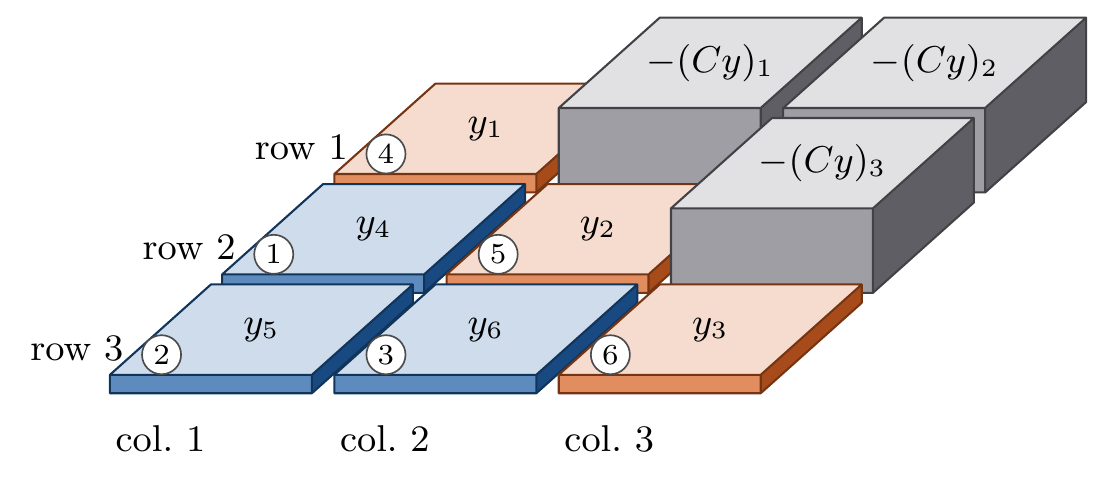
\includegraphics[width=0.66\textwidth]{figures/board.png}
\caption{The matrix $X_C(y)$ of~\eqref{eq:XC}. The six free positions carry the coordinates of $y$; the three raised positions carry $-Cy$. The circled numbers give the order~\eqref{eq:order} in which the corresponding columns of $C$ are fixed: the strictly lower positions first, then the diagonal.}
\label{fig:board}
\end{figure}

The search rests on a locality property. If $\supp y\subseteq S_d$, then $Cy=\sum_{k\in S_d}y_k\,C_{\ast k}$ involves only the columns of $C$ in $S_d$, so $X_C(y)$ is the same matrix for every $C$ extending a given node. We call a node of depth $d\ge1$ \emph{closed} if there is $y\in\F_3^6$ with $\supp y\subseteq S_d$, $y_{\sigma_d}=1$ and $X_C(y)^3=0$, for $C$ extending the node; by locality such a $y$ serves every extension at once.\footnote{Restricting to $y_{\sigma_d}=1$ loses nothing. A vector $y\ne0$ with support in $S_d$ has a largest $e\le d$ with $y_{\sigma_e}\ne0$; after multiplying by $\pm1$, which does not affect nilpotency, $y_{\sigma_e}=1$, and $y$ is a candidate at the ancestor of depth $e$.}

The tree is built from the root, the unique node of depth $0$: a node of depth $d<6$ that is not closed receives as children its $27$ extensions to depth $d+1$. Proposition~\ref{prop:finite} follows once every node of depth $6$ in this tree is closed. Indeed, given $C$, consider the nodes on the path from the root to the node of depth $6$ that $C$ determines; the first closed node on the path exists and lies in the tree, and its witness $y$ gives $X_C(y)^3=0$.

\begin{proposition}\label{prop:tree}
The tree has $3{,}109{,}888$ nodes, and every node of depth $6$ is closed. Table~\ref{tab:tree} and Figure~\ref{fig:tree} give the counts by depth.
\end{proposition}

\begin{table}[ht]
\centering
\begin{tabular}{@{}lrrrrrrr@{}}
\toprule
depth $d$ & $0$ & $1$ & $2$ & $3$ & $4$ & $5$ & $6$\\
\midrule
nodes & $1$ & $27$ & $486$ & $6{,}966$ & $48{,}627$ & $1{,}312{,}929$ & $1{,}740{,}852$\\
closed & -- & $9$ & $228$ & $5{,}165$ & $0$ & $1{,}248{,}453$ & $1{,}740{,}852$\\
\bottomrule
\end{tabular}
\medskip
\caption{The search tree of Proposition~\ref{prop:tree}. Each open node of depth $d<6$ has $27$ children.}
\label{tab:tree}
\end{table}

\begin{figure}[ht]
\centering
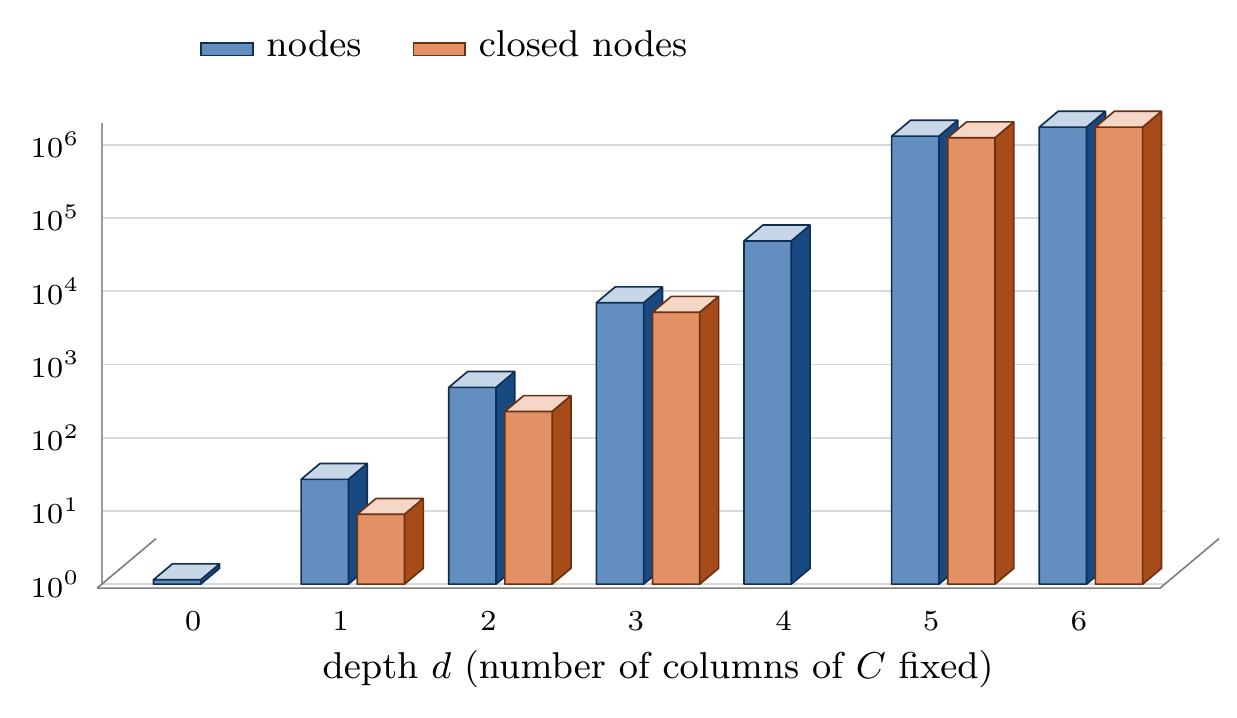
\includegraphics[width=0.72\textwidth]{figures/tree.png}
\caption{Nodes and closed nodes of the search tree by depth, on a logarithmic scale.}
\label{fig:tree}
\end{figure}

The shape of the tree has a simple explanation. While only lower columns are fixed ($d\le3$), the candidates $y$ are supported on the strictly lower positions, so $X_C(y)$ has zero diagonal and is nilpotent exactly when $c_2(X_C(y))=\det X_C(y)=0$; already three quarters of the nodes of depth $3$ close in this way. At depth $4$ the candidates have $y_1=1$ and no other diagonal entry, hence trace $1$, and no node closes. At depths $5$ and $6$ the trace condition can be met, and the remaining nodes close.

\subsection{Formal verification}\label{sec:lean}
The search tree, the soundness argument and the reduction of Section~\ref{sec:reduction} are formalised in Lean~4~\cite{MU} with Mathlib~\cite{Mathlib}; the development is archived with this paper~\cite{Ar}. It consists of three parts.
\begin{enumerate}[label=(\roman*),leftmargin=*]
\item A search function written in plain Lean, without Mathlib, which explores the tree above with the cube test of Lemma~\ref{lem:nil} written out entry by entry, together with a check that every candidate vector at depth $d$ is nonzero and supported on $S_d$.
\item A proof, by induction on the number of columns still to be fixed, that if the search function and the candidate check both return \emph{true}, then Proposition~\ref{prop:finite} holds.
\item A proof of Lemma~\ref{lem:graph} for subspaces in Mathlib's sense, with dimension given by \emph{finrank}, from which Theorem~A, the negation of Conjecture~\ref{conj:W} as a formal statement over all finite fields, and Theorem~B follow.
\end{enumerate}
The two Boolean equations of part (i) are evaluated by compiled code; this takes about four and a half minutes on one core. Lean records each such evaluation as an axiom asserting exactly the evaluated equation, so the trusted base consists of the Lean kernel, the three standard axioms (propositional extensionality, choice and soundness of quotients), and the Lean compiler for these two equations. The check of the $242$ matrices of $W_5$ is done by the kernel.

The development also contains Lemma~\ref{lem:shift}, the two statements of Lemma~\ref{lem:quadric} used later (the formula for $c_2$ and the fact that the radical is $FI$), Propositions~\ref{prop:cone} and~\ref{prop:identity} (the latter with Mathlib's Chevalley--Warning theorem), Proposition~\ref{prop:two} for every finite field, and Examples~\ref{ex:F2} and~\ref{ex:F5}, whose finite checks are again done by the kernel. These use only the three standard axioms. The one statement of the paper that is not formalised is the count of zeros of a quadric quoted after Proposition~\ref{prop:cone}.

\subsection{Independent computations}
Two exhaustive enumerations of a different kind confirm Theorem~A.

First, a six-dimensional subspace $W\le\M_3(\F_3)$ is the orthogonal complement $U^\perp$ of a three-dimensional $U\le\F_3^9$ for the standard dot product on matrix entries, and $U$ is the row space of a unique $3\times9$ matrix in reduced row echelon form. The subspace $W$ is nilpotent-free exactly when each of the $364$ lines of nonzero nilpotent matrices is not orthogonal to $U$. Running through all $\binom{9}{3}_3=678{,}468{,}820$ echelon matrices, no nilpotent-free $W$ occurs. (That there are $364=(3^6-1)/2$ such lines is the theorem of Fine and Herstein~\cite{FH} that $\M_n(\F_q)$ contains exactly $q^{n^2-n}$ nilpotent matrices.)

Second, if $\dim W=6$ then $W\cap\sll_3(\F_3)$ has dimension at least five, where $\sll_3$ denotes the trace-zero matrices. All $\binom 83_3=25{,}095{,}280$ five-dimensional subspaces of $\sll_3(\F_3)$ contain a nonzero nilpotent matrix, which is a second proof of Theorem~A that does not use Lemma~\ref{lem:graph}. The search tree has also been written again in C++, with the same node counts. The programs are archived with the paper~\cite{Ar}.

\section{Characteristic three}\label{sec:char3}

In this section $F=\F_q$ with $q=3^k$. Since $\tr I=3=0$, the identity lies in $\sll_3(F)$.

\begin{lemma}\label{lem:shift}
For $X\in\sll_3(F)$ and $a\in F$,
\[
c_2(X+aI)=c_2(X),\qquad \det(X+aI)=\det X+a^3+a\,c_2(X).
\]
\end{lemma}

\begin{proof}
The characteristic polynomial of $X$ is $\chi(t)=t^3+c_2(X)\,t-\det X$. In characteristic three $(t-a)^3=t^3-a^3$, so the characteristic polynomial of $X+aI$ is
\[
\chi(t-a)=t^3+c_2(X)\,t-\bigl(\det X+a^3+a\,c_2(X)\bigr),
\]
and the two identities can be read off.
\end{proof}

\begin{lemma}\label{lem:quadric}
On $\sll_3(F)$ one has $c_2(X)=\tr(X^2)$. The polar form of $c_2$ is $(X,Y)\mapsto 2\tr(XY)$, whose radical in $\sll_3(F)$ is the line $FI$. Hence $c_2$ induces a nondegenerate quadratic form $\bar c_2$ on the seven-dimensional space $V=\sll_3(F)/FI$.
\end{lemma}

\begin{proof}
Newton's identity $2c_2(X)=(\tr X)^2-\tr(X^2)$ gives $c_2(X)=-\tfrac12\tr(X^2)=\tr(X^2)$ on $\sll_3(F)$, because $-\tfrac12=1$ in $F$. The polar form is $c_2(X+Y)-c_2(X)-c_2(Y)=2\tr(XY)$. The trace form is nondegenerate on $\M_3(F)$, and the orthogonal complement of $\sll_3(F)=(FI)^\perp$ is $FI$; since $FI\subseteq\sll_3(F)$, the radical of the restriction to $\sll_3(F)$ is $FI$. The form is constant on cosets of $FI$ by Lemma~\ref{lem:shift}, and as $q$ is odd it is nondegenerate on the quotient.
\end{proof}

\begin{proposition}\label{prop:cone}
The quotient map $\sll_3(F)\to V$ restricts to a bijection from the set of nilpotent matrices in $\M_3(F)$ onto the set of zeros of $\bar c_2$.
\end{proposition}

\begin{proof}
A nilpotent matrix lies in $\sll_3(F)$ and has $c_2=0$ by Lemma~\ref{lem:nil}, so it maps to a zero of $\bar c_2$. Conversely let $X\in\sll_3(F)$ with $c_2(X)=0$. By Lemmas~\ref{lem:nil} and~\ref{lem:shift}, $X+aI$ is nilpotent exactly when $\det X+a^3=0$. The map $a\mapsto a^3$ is the Frobenius automorphism of $F$, so there is exactly one such $a$.
\end{proof}

A nondegenerate quadratic form in seven variables over $\F_q$ has exactly $q^6$ zeros~\cite[Chapter~6]{LN}, so Proposition~\ref{prop:cone} gives a short proof, for $n=3$ and $q$ a power of three, of the count $q^{n^2-n}$ of Fine and Herstein.

\begin{proposition}\label{prop:identity}
Let $U\le\sll_3(F)$ with $I\in U$ and $\dim U\ge4$. Then $U$ contains a nonzero nilpotent matrix. Consequently a nilpotent-free subspace of $\M_3(F)$ of dimension at least five does not contain $I$.
\end{proposition}

\begin{proof}
The image of $U$ in $V$ has dimension at least three, and the restriction of $\bar c_2$ to it is a quadratic form in at least three variables, which has a nonzero zero by the Chevalley--Warning theorem~\cite{Ch,Wa}. Choose $X\in U\setminus FI$ mapping to it. By Proposition~\ref{prop:cone} some $X+aI$ is nilpotent; it lies in $U$ because $I\in U$, and it is nonzero because $X\notin FI$. For the second statement, if $W$ is nilpotent-free with $\dim W\ge5$ and $I\in W$, apply the first to $U=W\cap\sll_3(F)$, which contains $I$ and has dimension at least $\dim W-1\ge4$.
\end{proof}

By Proposition~\ref{prop:identity}, the second computation of Section~\ref{sec:tree} need only consider five-dimensional subspaces $U\le\sll_3(\F_3)$ with $I\notin U$. For such $U$ the space $U\oplus FI$ maps onto a five-dimensional subspace $\bar U$ of $V$, every zero of $\bar c_2$ on $\bar U$ has exactly one nilpotent lift in $U\oplus FI$, and the question is whether one of these lifts lies in the hyperplane $U$. A nondegenerate form on $\bar U$ has $40$ projective zeros, and each lift lies in $U$ with a chance of one in three if the lifts behave independently. The enumeration agrees with this heuristic on average, the mean number of nilpotent lines being close to $40/3$, and shows how little room there is at the extreme: $1{,}872$ of the five-dimensional subspaces of $\sll_3(\F_3)$ contain exactly one line of nilpotent matrices. Theorem~A therefore cannot follow from a counting argument alone, and we do not know a proof that avoids the computation.

\section{Fields where the conjecture holds}\label{sec:holds}

\begin{proposition}\label{prop:two}
Conjecture~\ref{conj:W} holds for $n\le2$ and every finite field $F$.
\end{proposition}

\begin{proof}
For $n=1$ take $W=F$. For $n=2$ choose $M\in\M_2(F)$ such that the binary quadratic form $u\mapsto u^{\mathsf T}Mu$ has no nonzero zero; such forms exist over every finite field, for instance the norm form of $\F_{q^2}$ over $F$ written in a basis. Let $J=\left(\begin{smallmatrix}0&-1\\1&0\end{smallmatrix}\right)$ and $W=\{X:\tr(JMX)=0\}$, a space of dimension $3=2^2-\binom22$. A nonzero nilpotent $X\in\M_2(F)$ has rank one and square zero, so $X=uv^{\mathsf T}$ with $u,v\ne0$ and $v^{\mathsf T}u=0$, that is $v=\lambda Ju$ with $\lambda\ne0$. Then $\tr(JMX)=v^{\mathsf T}JMu=\lambda\,u^{\mathsf T}J^{\mathsf T}JMu=\lambda\,u^{\mathsf T}Mu\ne0$, so $X\notin W$.
\end{proof}

\begin{example}\label{ex:F2}
Over $\F_2$ the space
\[
\left\{\begin{pmatrix} a&b+d+e&a+e+f\\ d&b&b+f\\ e&f&c\end{pmatrix} : a,\dots,f\in\F_2\right\}
\]
is six-dimensional and nilpotent-free, so the conjecture holds for $n=3$ over $\F_2$. By Lemma~\ref{lem:graph} a nilpotent-free six-dimensional subspace is $\{X_C(y)\}$ for a unique $C$, and running through the $2^{18}$ matrices $C\in\F_2^{3\times6}$ shows that exactly $128$ of the $\binom93_2=788{,}035$ six-dimensional subspaces of $\M_3(\F_2)$ are nilpotent-free.
\end{example}

\begin{example}\label{ex:F5}
Over $\F_5$ the space of matrices
\[
\begin{pmatrix} a&3a+4b+d+2e+2f&3a+3b+3e+3f\\ d&b&a+4b+c+3d+3f\\ e&f&c\end{pmatrix},\qquad a,\dots,f\in\F_5,
\]
is six-dimensional and nilpotent-free, as a check of its $5^6-1$ nonzero elements shows. So the conjecture holds for $n=3$ over $\F_5$.
\end{example}

For $q\in\{4,7,8,9\}$ we do not know whether $\M_3(\F_q)$ has a nilpotent-free subspace of dimension six. By Lemma~\ref{lem:graph} such a subspace is $\{X_C(y)\}$ for some $C\in\F_q^{3\times6}$, and a local search over $C$, which found the examples over $\F_2$ and $\F_5$, found none for these fields in twenty-five minutes each. We draw no conclusion from this.

\section{Remarks and questions}\label{sec:questions}

\begin{remark}\label{rem:transfer}
Theorem~A does not rule out a duality proof of the Gerstenhaber--Serezhkin bound over $\overline{\F}_3$. A space $N$ of nilpotent matrices over $\overline{\F}_3$ is spanned by finitely many matrices, whose entries lie in some $\F_{3^k}$; their span over $\F_{3^m}$ for any multiple $m$ of $k$ consists of nilpotent matrices and has the same dimension as $N$. It therefore suffices to have nilpotent-free spaces of dimension $n^2-\binom n2$ over $\F_{3^m}$ for some multiple $m$ of every $k$. Theorem~A only removes $m=1$.
\end{remark}

\begin{question}
Does $\M_3(\F_9)$ contain a nilpotent-free subspace of dimension six? More generally, for which $n$ and $q$ is the largest dimension of a nilpotent-free subspace of $\M_n(\F_q)$ smaller than $n^2-\binom n2$?
\end{question}

Proposition~\ref{prop:identity} holds over every field of characteristic three, and a similar but weaker phenomenon is available whenever the characteristic divides $n$, since then $I\in\sll_n$. It would be interesting to know whether the conjecture fails for other pairs $(n,q)$ with $p\mid n$, or whether $(3,\F_3)$ is an isolated exception.

\subsection*{Data availability}
The Lean~4 development, the programs of Section~\ref{sec:tree} and their outputs are archived with the source of this paper~\cite{Ar}.

\subsection*{Use of generative AI}
During the preparation of this work the author used Claude (Anthropic) to search the literature, to run and check the computations and the formal proofs, and to draft the text. The author checked every step of the proofs and every reference, and takes full responsibility for the content.

\begin{thebibliography}{99}

\bibitem{Ar}
D.~Bhattacharjee, \emph{Nilpotent-free spaces of $3\times3$ matrices over $\F_3$: paper, Lean~4 development and computations}, 2026. \url{https://github.com/creelie/congenial-waddle}

\bibitem{Ch}
C.~Chevalley, \emph{D\'emonstration d'une hypoth\`ese de M.~Artin}, Abh. Math. Sem. Univ. Hamburg \textbf{11} (1935), 73--75. \doi{10.1007/BF02940714}

\bibitem{Di}
J.~Dieudonn\'e, \emph{Sur une g\'en\'eralisation du groupe orthogonal \`a quatre variables}, Arch. Math. \textbf{1} (1949), 282--287. \doi{10.1007/BF02038756}

\bibitem{dSP}
C.~de Seguins Pazzis, \emph{On Gerstenhaber's theorem for spaces of nilpotent matrices over a skew field}, Linear Algebra Appl. \textbf{438} (2013), 4426--4438. \doi{10.1016/j.laa.2013.01.035}

\bibitem{FH}
N.~J. Fine and I.~N. Herstein, \emph{The probability that a matrix be nilpotent}, Illinois J. Math. \textbf{2} (1958), 499--504. \doi{10.1215/ijm/1255454112}

\bibitem{Ge}
M.~Gerstenhaber, \emph{On nilalgebras and linear varieties of nilpotent matrices.~I}, Amer. J. Math. \textbf{80} (1958), 614--622. \doi{10.2307/2372773}

\bibitem{LN}
R.~Lidl and H.~Niederreiter, \emph{Finite Fields}, 2nd ed., Encyclopedia Math. Appl. \textbf{20}, Cambridge University Press, Cambridge, 1997. \doi{10.1017/CBO9780511525926}

\bibitem{Mathlib}
The mathlib Community, \emph{The Lean mathematical library}, in: Proceedings of the 9th ACM SIGPLAN International Conference on Certified Programs and Proofs (CPP 2020), ACM, 2020, 367--381. \doi{10.1145/3372885.3373824}

\bibitem{Me}
R.~Meshulam, \emph{On the maximal rank in a subspace of matrices}, Quart. J. Math. Oxford Ser.~(2) \textbf{36} (1985), 225--229. \doi{10.1093/qmath/36.2.225}

\bibitem{MU}
L.~de Moura and S.~Ullrich, \emph{The Lean~4 theorem prover and programming language}, in: Automated Deduction (CADE 28), Lecture Notes in Comput. Sci. \textbf{12699}, Springer, 2021, 625--635. \doi{10.1007/978-3-030-79876-5_37}

\bibitem{Se}
V.~N. Serezhkin, \emph{Linear transformations preserving nilpotency}, Vests\={\i} Akad. Navuk BSSR Ser. F\={\i}z.-Mat. Navuk (1985), no.~6, 46--50 (Russian).

\bibitem{Wa}
E.~Warning, \emph{Bemerkung zur vorstehenden Arbeit von Herrn Chevalley}, Abh. Math. Sem. Univ. Hamburg \textbf{11} (1935), 76--83. \doi{10.1007/BF02940715}

\bibitem{Wi}
Y.~Wigderson, \emph{Duality for matrix space questions}, preprint, 2026, to appear in Amer. Math. Monthly. \href{https://arxiv.org/abs/2609.29177}{\nolinkurl{arXiv:2609.29177}}

\end{thebibliography}

\end{document}
